\aufgabe 1

\paragraph{a)}\mbox{} \\

Das in der Aufgabe beschriebene Model ist als Typ LHA II des Linearen Hybrid Automaten unterzuordnen. Die Ableitungen von a und b sind dabei weder Konstanten oder Intervalle, welche dem Typen LHA I unterzuordnen wären. Es handelt stattdessen bei sämtlichen Ableitungen um Funktionen, welche zu nicht linearen Veränderungen über Zeit führen. 

\paragraph{b)}\mbox{} \\

$$Hier\ Bild\ der\ Automaten\ und\ Networks\ und\ so$$

\paragraph{c)}\mbox{} \\


	$a==5000 \ \&\\
	b==5000 \ \& \\
	discharging\_rate==200 \ \& \\
	charging\_rate==-100 \ \& \\
	g==0 \ \& \\
	min\_charge==10 \ \& \\
	max\_charge==10 \ \& \\
	min\_discharge==10 \ \& \\ 
	max\_discharge==10 \ \& \\
	t\_charge==0 \ \& \\
	t\_discharge==0 \ \& \\
	loc(KineticBatteryModel\_1)==normal\_charging \ \& \\
	loc(controller\_1)==charging \\$		


\paragraph{d)}\mbox{} \\

\begin{figure}[H]
	\centering
	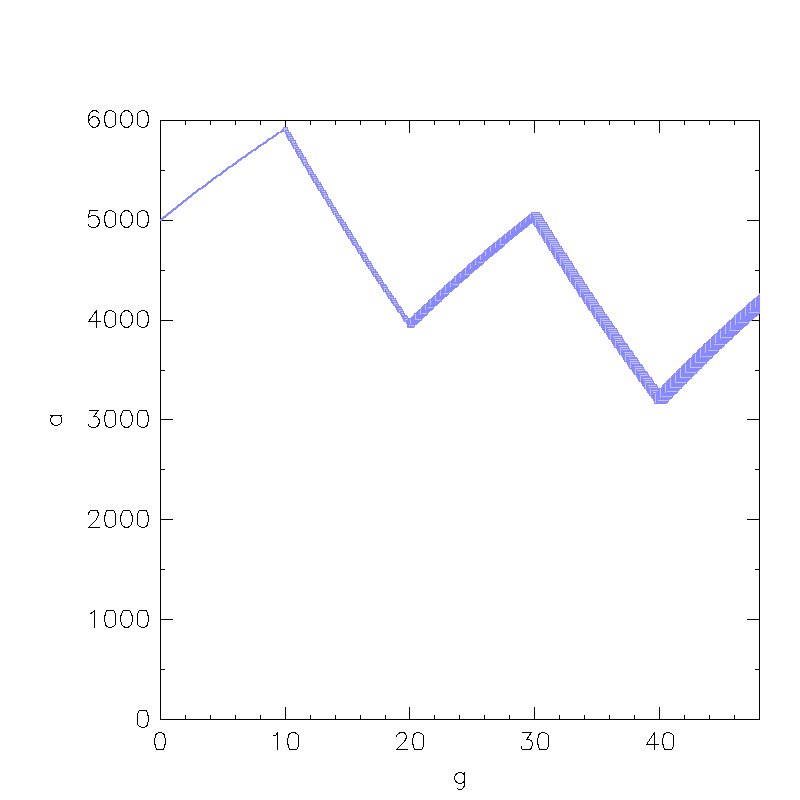
\includegraphics[width=0.8\textwidth]{Aufgabe_d).png}
\end{figure}

In dieser Abbildung ist in den beginnenden 10 Sekunden ein Ladevorgang in $a$ zu sehen. Sobald jedoch die Anforderung $a>b$ erfüllt ist, wird durch den Recovery Effect Ladung von $a$ an $b$ abgegeben. Aus diesem Grund ist nach 10 Sekunden ein Abfall zu erkennen, wodurch $a$ nicht vollständig bis 6000 aufgeladen wird. 


Ist die Anforderung $a>b$ im weiteren Verlauf erneut nicht erfüllt, kommt es zu einer Umkehrung des Recovery Effects, wodurch $a$ erneut aufgeladen wird. Dieser Vorgang wechselt sich entsprechend ab und es kommt zu Wiederholungen, wie an dem Auf- und Abstieg von $a$ im obigen Graphen zu sehen ist. 

\paragraph{e)}\mbox{} \\

\begin{figure}[H]
	\centering
	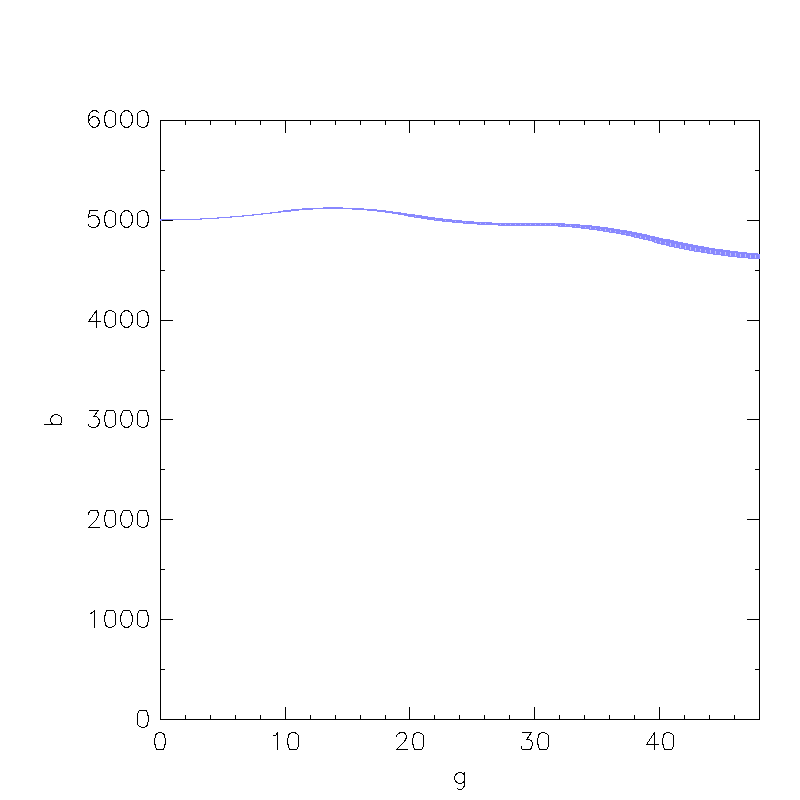
\includegraphics[width=0.8\textwidth]{Aufgabe_e).png}
\end{figure}

Wie schon in Aufgabe d) zu erkennen war, ist auch in diesem Graphen der Recovery Effect widergespiegelt. Je größer der Abstand zu $a$ wird umso stärker wird dieser Effekt. Durch die Anforderung $a>b$ wird $b$ weiterhin im dem Punkt geladen indem a bereits entladen ist. Der Graph hat weiterhin einen Scheitelpunkt sobald der Fall $a=b$ eintritt. Im Anschluss tritt der Fall $a<b$ ein, wodurch Ladung von $b$ abgegeben wird. Analog zur vorherigen Aufgabe wiederholt sich der Vorgang. 

\paragraph{f)}\mbox{} \\

\begin{figure}[H]
	\centering
	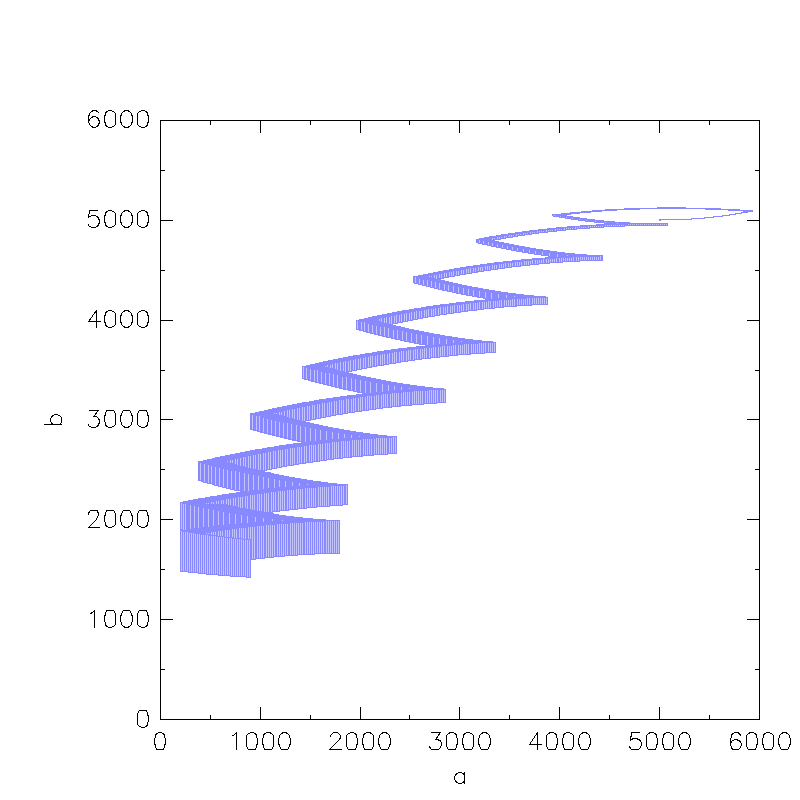
\includegraphics[width=0.8\textwidth]{Aufgabe_f).png}
\end{figure}

\paragraph{g)}\mbox{} \\
\begin{minipage}[t]{0.5\textwidth} 
	\begin{figure}[H]
		\centering
		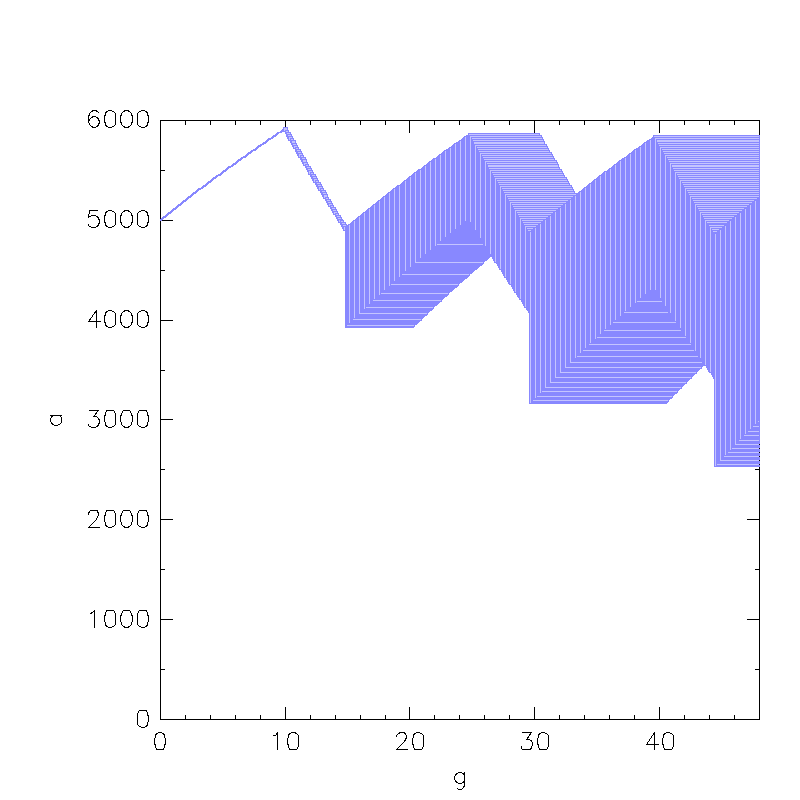
\includegraphics[width=0.8\textwidth]{Aufgabe_g1).png}
	\end{figure}
\end{minipage}
\hfill
\begin{minipage}[t]{0.5\textwidth} 
	\begin{figure}[H]
		\centering
		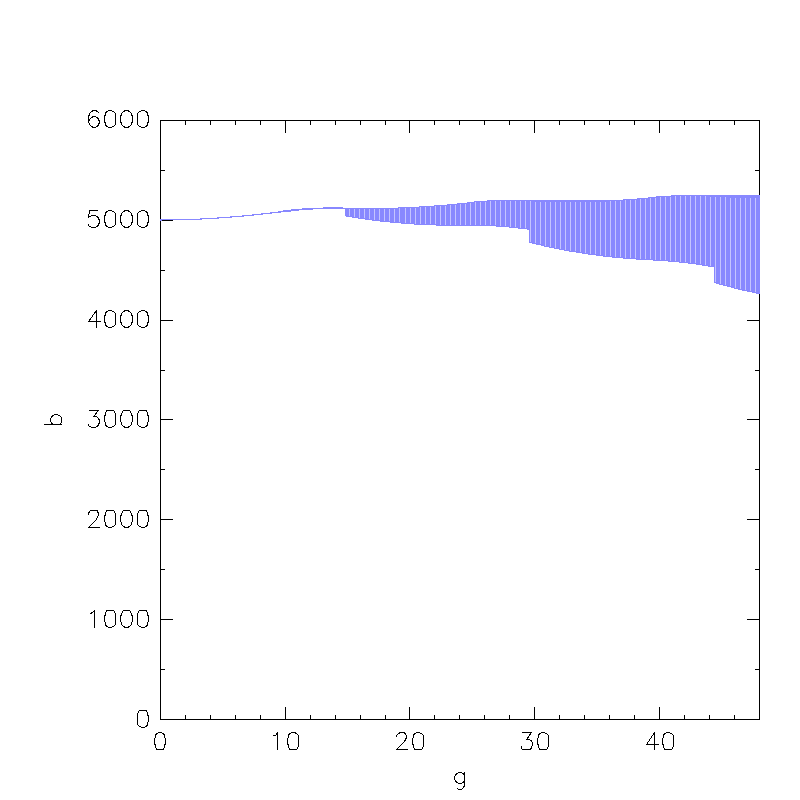
\includegraphics[width=0.8\textwidth]{Aufgabe_g2).png}
	\end{figure}
\end{minipage}

\paragraph{h)}\mbox{} \\

\begin{minipage}[t]{0.5\textwidth} 
	\begin{figure}[H]
		\centering
		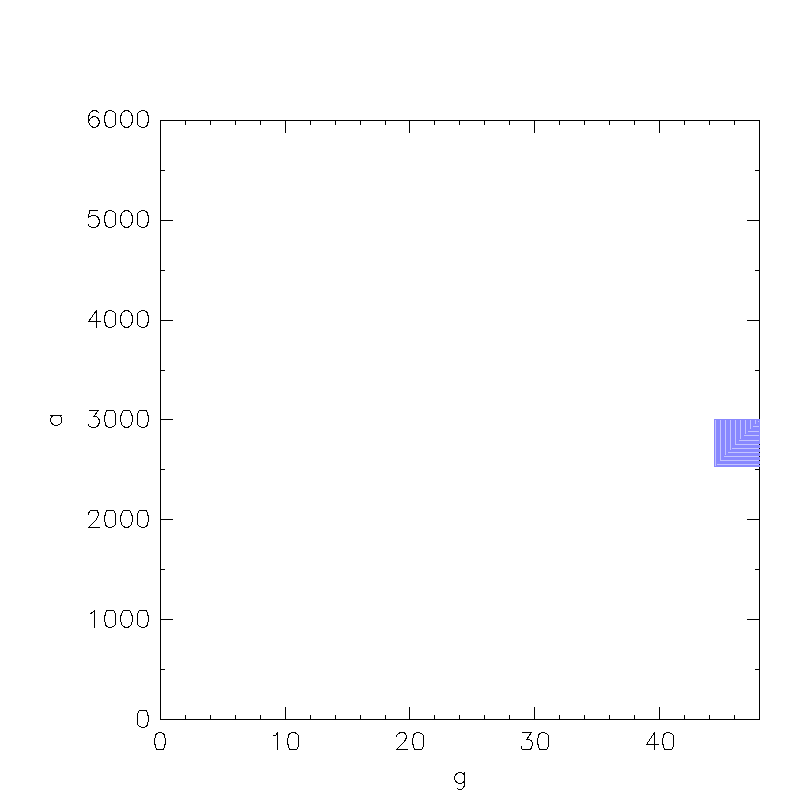
\includegraphics[width=0.8\textwidth]{Aufgabe_h1).png}
	\end{figure}
\end{minipage}
\hfill
\begin{minipage}[t]{0.5\textwidth} 
	\begin{figure}[H]
		\centering
		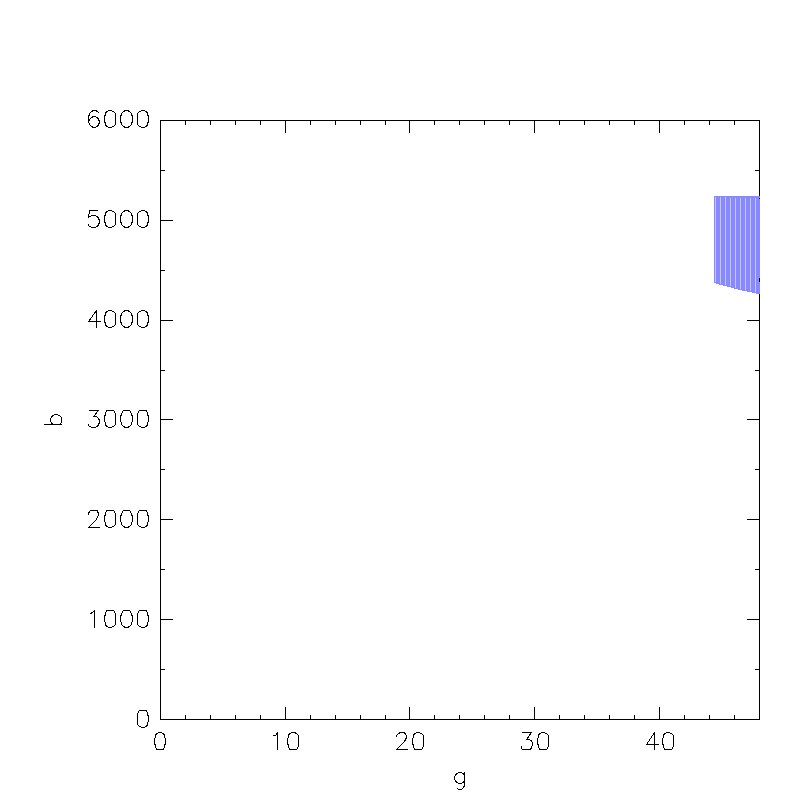
\includegraphics[width=0.8\textwidth]{Aufgabe_h2).png}
	\end{figure}
\end{minipage}

\paragraph{i)}\mbox{} \\

\paragraph{j)}\mbox{} \\
	\begin{figure}[H]
	\centering
	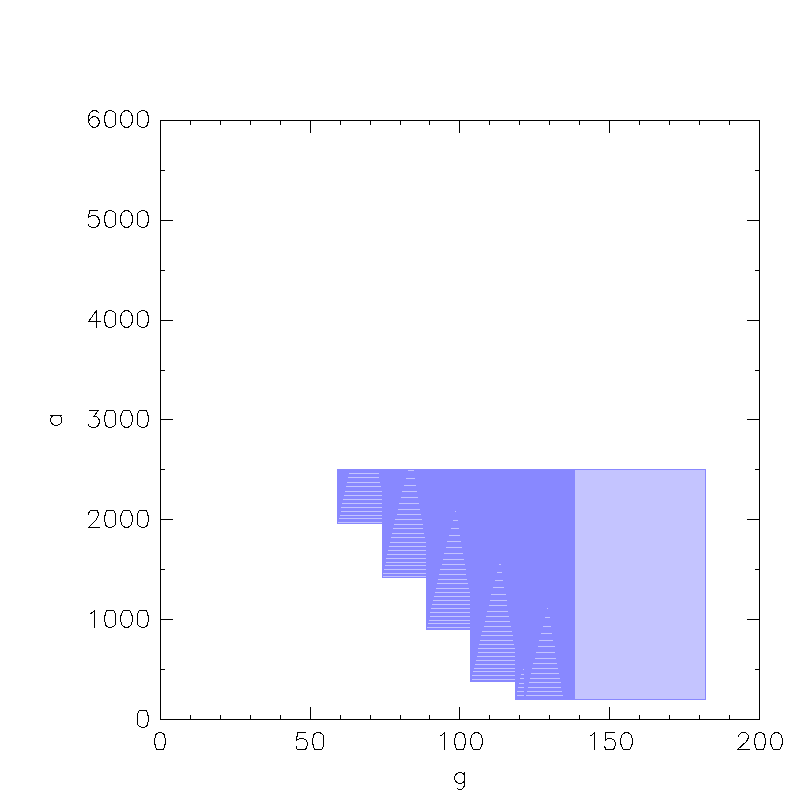
\includegraphics[width=0.8\textwidth]{Aufgabe_j).png}
\end{figure}

\paragraph{k)}\mbox{} \\

	\begin{figure}[H]
	\centering
	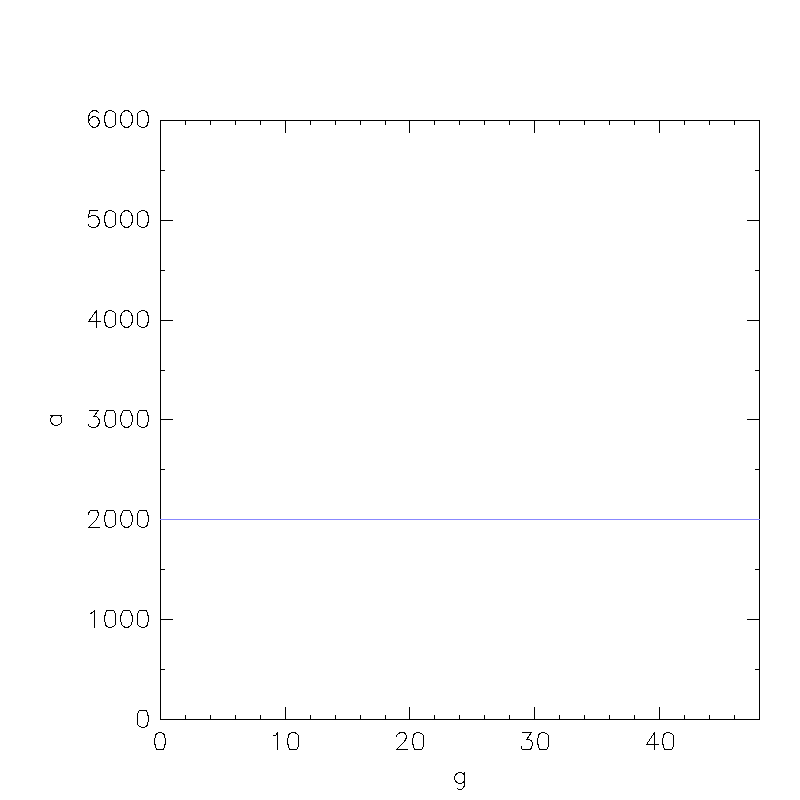
\includegraphics[width=0.8\textwidth]{Aufgabe_k).png}
\end{figure}